\textbf{P2)} \textcolor{red}{[Prueba 1 - 2025-20]} Una rueda de radio $R$, masa $M$ y momento de inercia con respecto a centro de masa
\[
I_{cm}=\frac{MR^2}{2},
\]
rueda perfectamente (sin deslizamiento) sobre superficie rugosa, y es tirado por un cordel atado a su eje. Este cordel pasa a través de una polea de radio $r$ y momento de inercia $I_O$, haciéndola rodar (sin deslizamiento), y en su otro extremo tiene un cilindro de masa $m$.

\begin{enumerate}[a)]
\item Encuentre dos relaciones entre $v_{cm}$, la velocidad angular de la rueda $\omega$, y la velocidad angular de la polea $\omega_1$.
\item Dibuje los DCL de la rueda, de la polea y del cilindro.
\item Escriba las ecuaciones de movimiento relevantes.
\item Calcule la aceleración del centro de la rueda $a$.
\end{enumerate}

\begin{center}
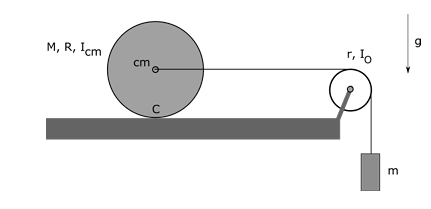
\includegraphics[width=0.55\textwidth]{imagenes/ayudantia_4_p2.png}
\end{center}

\vspace{0.2cm}
\textbf{Solucion}

Rueda, polea y cilindro:

\begin{enumerate}[a)]
\item Nos podemos dar cuenta que la rueda y el cilindro se mueven con la misma velocidad $v$ y aceleracion $a$. Como se trata de rodadura perfecta en la rueda y la polea, la rueda gira con velocidad angular:
\[
\omega=\frac{v}{R}
\qquad\Rightarrow\qquad
\alpha=\frac{a}{R}.
\]
Y la polea (que rueda sobre el cordel) gira con velocidad angular:
\[
\omega_1=\frac{v}{r}
\qquad\Rightarrow\qquad
\alpha_1=\frac{a}{r}.
\]


\item \textbf{DCL de la rueda:} 
\begin{itemize}
\item peso $Mg$ aplicado en centro hacia abajo;
\item normal $N$ aplicada en punto de contacto hacia arriba;
\item roce $f$ aplicado en punto de contacto hacia izquierda;
\item tension $T_1$ aplicada en centro hacia la derecha.
\end{itemize}
DC de la rueda: $a$ hacia la derecha, $\alpha$ sentido horario.

\textbf{DCL de la polea:}
\begin{itemize}
\item reaccion horizontal $H$ aplicada en centro hacia derecha;
\item reaccion vertical $V$ aplicada en centro hacia arriba;
\item tension $T_1$ aplicada en borde superior hacia izquierda;
\item tension $T_2$ aplicada en borde derecho hacia abajo.
\end{itemize}
(No se indicaba el peso. Lo relevante son las tensiones. En general $T_1\neq T_2$.)
DC de polea: $\alpha_1$ sentido horario.

\textbf{DCL del peso:}
\begin{itemize}
\item peso $mg$ hacia abajo;
\item tension $T_2$ hacia arriba.
\end{itemize}
DC de peso: $a$ hacia abajo.


\item \textbf{Ecuaciones}

Las ecuaciones de movimiento relevantes (para los torques sobre la rueda usamos su centro como punto de referencia):
\[
-f+T_1=Ma,
\]
\[
N-Mg=0,
\]
\[
Rf=\frac{MR^2}{2}\,\alpha,
\]
\[
-rT_1+rT_2=I_O\alpha_1,
\]
\[
mg-T_2=ma.
\]

(No usamos las ecuaciones de fuerza sobre la polea.) Contando las ecuaciones de $\alpha$ y $\alpha_1$, tenemos en total 7 ecuaciones para 7 incognitas ($T_1,T_2,f,N,a,\alpha,\alpha_1$). Descartamos la segunda ecuacion porque no nos interesa $N$.

Reemplazamos $\alpha=a/R$ y $\alpha_1=a/r$ para llegar a 4 ecuaciones con 4 incognitas. Multiplicando por $R$ la primera ecuacion, y por $r$ la ultima ecuacion, y sumando primera con tercera (para eliminar $f$), y cuarta con quinta (para eliminar $T_2$):
\[
RT_1=\left(MR+\frac{MR}{2}\right)a,
\]
\[
rmg-rT_1=\left(\frac{I_O}{r}+mr\right)a.
\]

Dos ecuaciones para dos incognitas. Combinando estas dos ecuaciones llegamos a:
\[
Rrmg=\left(\frac{3}{2}MRr+\frac{I_OR}{r}+mRr\right)a
\qquad\Rightarrow\qquad
a=\frac{Rrmg}{\frac{3}{2}MRr+\frac{I_OR}{r}+mRr}.
\]

Equivalentemente,
\[
\boxed{a=\frac{mg}{m+\frac{3}{2}M+\frac{I_O}{r^2}}}.
\]
\end{enumerate}
